%include part: see main.beamer.tex and main.article.tex
\mode<article>{\usepackage{fullpage}}
\mode<presentation>{
    %оформление
    \usetheme{Madrid} %%Madrid, CambridgeUS, Malmoe, Singapore, Berlin
    \useoutertheme{shadow}
} 


\usepackage[russian]{babel}
\usepackage[utf8]{inputenc}
\usepackage{graphicx}


\title[Презентации в beamer]{Оформление презентаций в beamer}
\date{\today}
\author[М.~М.~Шихов]{Михаил Шихов \\ \texttt{\underline{kafevm@mail.ru}}}


\begin{document}


%титул и содержание статьи
\mode<article>{\maketitle\tableofcontents}
%команда mode определяет в каком отображении появится агрумент: в данном случае только в статье!

%титул и содержание презентации
\frame<presentation>{\titlepage}
\begin{frame}<presentation>[allowframebreaks]
    \frametitle{Содержание}
    \tableofcontents
\end{frame}
%благодаря аргументу presentation в угловых скобках команды frame данные фреймы не появяться в статье


\section{Основные моменты}

Все, что не в окружении frame, в презентацию не попадает, но попадает в статью!


\subsection{Теоремы и оверлеи}

Агрументы в угловых скобках команд item, alert, uncover позволяют указывать через запятую диапазоны оверлеев, к которым они применимы.
\begin{frame}
    \frametitle{Пример оверлея}
    \framesubtitle{Евклид: простых чисел бесконечно много}
    
    \begin{theorem}
        Простых чисел бесконечно много.
    \end{theorem}
    \begin{proof}
        \begin{enumerate}
            \item<1-> Пусть \alert<1,4>{$p$ --- наибольшее из простых} чисел.
            \item<2-> Пусть $q=p!$ произведение всех чисел, меньших $p$.
            \item<3-> Тогда $q + 1$ \alert<3>{не делится} ни на одно из них.
            \item<1-> Поэтому $q + 1$ \alert<4>{простое, большее чем $p$}.\qedhere
        \end{enumerate}
    \end{proof}
    \uncover<4->{Использовано доказательство от противного.}
\end{frame}


\subsection{Вставка изображений}

В статье изображение \ref{pict:AccessControl} <<уплывет>> как это принято в \LaTeX.

\begin{frame}
    \frametitle{Вставка изображения из внешнего файла}
    \framesubtitle{Монитор доступа}
    
    \begin{figure}
        \begin{center}
            \mode<presentation>{ 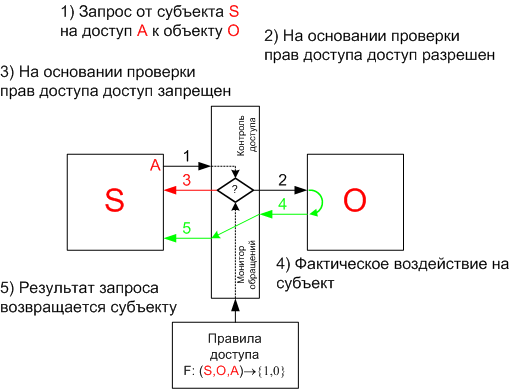
\includegraphics[height=.7\textheight]{pict/AccessControl} }
            \mode<article>{ 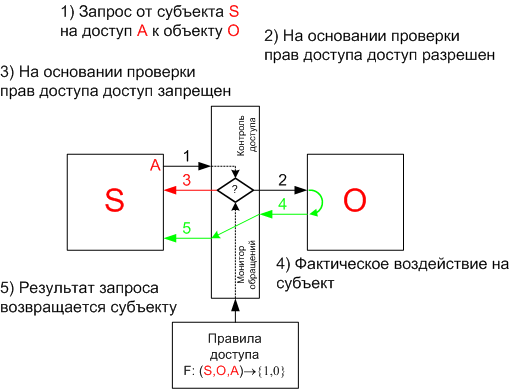
\includegraphics[width=.7\textwidth]{pict/AccessControl} } 
            
            \caption{Монитор доступа}
            \label{pict:AccessControl}
        \end{center}
    \end{figure} 
    \mode<article>{см. рис. \ref{pict:AccessControl}}
\end{frame}


\subsection{Колонки}

\begin{frame}
    \frametitle{Множество колонок}
    \framesubtitle{Пример оформления вопросов теста}
    
    \begin{enumerate}

        \item \label{enumer:infoProperties} Назовите основные свойства информации с точки зрения её защиты. В отношении каких объектов они проявляются?
        \item Назовите:
        \begin{columns}
            \column{.47\textwidth}
                \begin{block}{Первый вариант}
                    Основные \alert{точки зрения} на информацию
                \end{block}
            
            \column{.47\textwidth}
                \begin{block}{Второй вариант}
                    Основные \alert{подходы} к количественной оценке свойств информации.
                \end{block}
        \end{columns}
    
        \item Задача. Совместная информация двух независимых событий равна 7 бит. Вероятность одного из событий: 0.125. Опредедите вероятность второго события.
    \end{enumerate}
\end{frame}


\section{Оформляем код}

\subsection{Красивый semiverbatim} 

\begin{frame}[fragile]
    \frametitle{Оформление программного кода:semiverbatim}
    \framesubtitle{Паттерн <<одиночка>>}
\begin{semiverbatim}
\uncover<1->{\alert<0>{class Singleton \{ }}
\uncover<2->{\alert<2>{public:     static Singleton& \alert{Instance}() \{ }}
\uncover<3->{\alert<3>{                if (!pInstance_) }}
\uncover<3->{\alert<3>{                    pInstance_ = new Singleton(); }}
\uncover<3->{\alert<3>{                return *pInstance_; }}
\uncover<2->{\alert<2>{            \} }}
\uncover<5->{\alert<5>{            void foo() \{...\} //Не статические  }}
\uncover<5->{\alert<5>{                             //член-функции и член-данные! }}
\uncover<3->{\alert<3>{private:    static Singleton *pInstance_ = 0; }}
\uncover<4->{\alert<4>{            Singleton(); }}
\uncover<4->{\alert<4>{            Singleton(const Singleton&); }}
\uncover<4->{\alert<4>{            Singleton& operator=(const Singleton&); }}
\uncover<4->{\alert<4>{            ~Singleton(); }}
\uncover<1->{\alert<0>{\} }}
\end{semiverbatim}
\end{frame}


\section{Библиография}

Библиографию, конечно, можно определить и не используя bibtex!

\begin{frame}
    \frametitle{Источники}
    
    Из книг по \LaTeXe\ можно рекомендовать \cite{bib:cotelnikov,bib:baldin}. Про \TeX\ от автора \cite{bib:knuth:AllAbout}.
\end{frame}


%слайд раскладывается на несколько: allowframebreaks
\begin{frame}[allowframebreaks]{Библиография}

    \bibliographystyle{gost780u}
    \bibliography{bibliobase}
\end{frame}




\end{document}